% Downsampling diagram: top row = all filled samples (original),
% bottom row = alternating filled/empty (factor-2 downsampled).
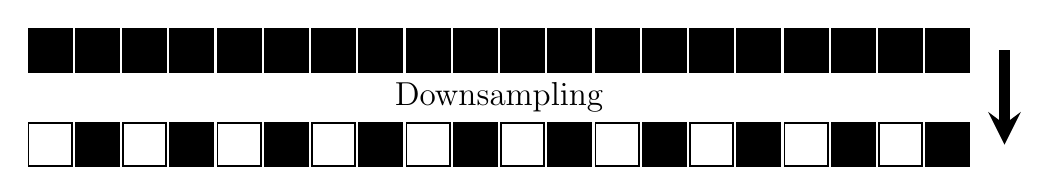
\begin{tikzpicture}[
    box/.style={draw=black, fill=#1, minimum size=0.55cm, inner sep=0pt, line width=0.6pt},
    x=0.6cm, y=0.6cm
]

\def\N{20}       % number of samples
\def\gap{0.05}   % inter-box gap (fraction of x unit — handled by minimum size)

% ── Top row: original signal (all filled) ────────────────────────────────────
\foreach \i in {1,...,\N} {
    \node[box=black] at (\i, 1.6) {};
}

% ── Label ────────────────────────────────────────────────────────────────────
\node[font=\large] at ({(\N+1)/2}, 0.6) {Downsampling};

% ── Arrow below label ────────────────────────────────────────────────────────
\draw[-stealth, line width=4pt] ({\N+1.2}, 1.6) -- ({\N+1.2}, -0.4);

% ── Bottom row: every other sample kept (black), rest dropped (white) ────────
\foreach \i in {1,...,\N} {
    \pgfmathparse{mod(\i,2)==0 ? "black" : "white"}
    \edef\fillcol{\pgfmathresult}
    \node[box=\fillcol] at (\i, -0.4) {};
}

\end{tikzpicture}
